% Hoda Abbasi
% 13 May 2016

\documentclass{report}
\input Latex_macros/Definitionen.tex
\usepackage{a4}
\usepackage{graphicx}
\usepackage{tikz-qtree}
\usepackage[active]{srcltx}
\usepackage[all]{xy}
\usepackage{enumerate}

\nc{\Dt}[1]{\mc{F}_{#1}} 
\nc{\tsubres}{\xrightarrow{\text{sfsR}}}
\nc{\tsubresk}[1]{\xrightarrow{\text{sfsR}}_{\!#1}}
\DMO{\saturate}{S}

\begin{document}
\title{Thesis Proposal: 
       }

\author{Hoda Abbasi\\
        PhD Candidate\\
        Computer Science Department\\
        Swansea University\\}
\maketitle

%%%%%%%%%%%%%%%%%%%%%%%%%%%%%%%%%%%%%%%%%%%%%%%%%%%%%%%%%%

\begin{abstract}
This proposal deals with two different aspects of SAT problem and particularly unsatisfiable problems. 

There are various measures for representing the complexity of SAT problems called ``hardness measures''. In the first part of this proposal, we review two measures of the hardness for clause-sets (``tree-hardness'' and ``width-hardness'') and a game characterisation for these measures. This game is performed by two players for a clause-set $F$ and has an ``optimal value'' corresponds to the hardness of $F$. Then, we use this game for obtaining the hardness of some graphs that are called Tseitin graphs. ?????????

The second part????????

The first chapter is dedicated to explain basic concepts and preliminaries. In chapter two, two hardness measures of clause-sets are introduced. Then, they are characterised by a game. Afterwards, the Tseitin clause-set (which is obtained from the Tseitin graph) is explained and the game is applied to them in order to obtain the hardness. Finally, ???

Chapter three explains ?????????
\end{abstract}

\tableofcontents
%%%%%%%%%%%%%%%%%%%%%%%%%%%%%%%%%%%%%%%%%%%%%%%%%%%%%%%%%%
\chapter{Preliminaries}
\label{cha:Preliminaries}

In this chapter, we use basic concepts according to \cite{h8, h18,h9}. 

\section{Clause-sets}
\label{sec:Clause-sets}

The infinite set of variables is denoted by $\Va$. A partial assignment $\vp$ is a map which assigns a unique value in $\set{0,1}$ to some elements of a finite set of variables. The domain of this map is a set of variables denoted by $\var(\vp)$. The set of all partial assignments is indicated by $\Pass$ and for $V \in \pote(\Va)$, $\Tass(V)$ is the set of total assignments over $V$. The empty partial assignment is denoted by $\epa:= \es \in \Pass$. For a partial assignment $\vp \in \Pass$, the number of variables is defined as $n(\vp):=\abs{\var(\vp)}$. For two partial assignments $\vp, \psi \in \Pass$, the composition operation is defined as $\vp \circ \psi := \psi \cup (\vp \sm \var(\psi)) \in \Pass$ which is the union of their variables if they do not conflict. In the case of conflicting variables, the second assignment is considered. This operation has associative property and it is commutative if $\vp, \psi$ do not clash.

A literal is a pair $(v,\ve)$ with $\var((v,\ve)):=v \in \Va$ (the underlying variable) and $\val((v,\ve)):=\ve \in \set{0,1}$. The set of all literals is $\Lit$. Two literals $x, y \in \Lit$ clash if they have a same variable but different values. For a set $L \sse \Lit$ we define $\var(L) := \set{\var(x) :x \in L}$, $\lit(L):= \set{x \in \Lit : \var(x) \in \var(L)}$ and $\ol{L} := \lit(L) \sm L$. A clause is defined as a finite and clash-free set of literals. The set of all clauses is denoted by $\Cl$ and $\bot := \es \in \Cl$ is the empty clause. The length (width) of a clause $C$ is the number of variables in $C$.

A clause-set is a finite set of clauses and $\Cls$ is the set of all clause-sets. The empty clause-set is indicated by $\top := \es \in \Cls$. For $F \in \Cls$ we define $\var(F) := \bc_{C \in F} \var(C) \in \pote(\Va)$ and $\lit(F) := \var(F) \cup \ol{\var(F)}$. The number of variables in $F$ is denoted by $n(F) := \abs{\var(F)} \in \NNZ$ and the number of clauses is $c(F) := \abs{F} \in \NNZ$. The number of literal occurrences in $F$ is also denoted by $\ell(F) := \sum_{C \in F} \abs{C} \in \NNZ$. If the union of literals occurring in $F$ is indicated by $\bigcup F \subset \Lit$, then a ``pure'' literal for $F \in \Cls$ is defined as $x \in \bigcup F$ and $\ol{x} \not \in \bigcup F$. A clause-set $F$ is called $k-\Cls$ if every clause in $F$ has length (width) at most $k$. A full clause $C$  for a clause-set $F$ is defined as $C \in F$ and $\var(C) = \var(F)$, and a clause-set $F$ is called full if every clause of $F$ is full. The full clause-set for a finite set of variables $V$ is denoted by $A(V)$. 

\begin{examp}\label{exp:An}
If $A(V)$ for $V=\set{1,..., n}$ is indicated by $A_n$ then $A_0 = \set{\bot}$, $A_1 = \set{\set{1},\set{-1}}$ and $A_2 = \set{\set{-1,-2},\set{-1,2},\set{1,-2},\set{1,2}}$.
\end{examp}

Partial assignments are extended from variables to literals using $\vp(\ol{v})=\ol{\vp(v)}$. The operation of a partial assignment on a clause-set is defined as $\vp * F := \set{C \sm \vp : C \in F \wedge C \cap \ol{\vp} = \es} \in \Cls$. This means removing all clauses having at least one literal with $\vp (x)=1$ and then, removing from all clauses the literals with $\vp (x)=0$. For a clause $C$, the partial assignment $\vp_C$ sets precisely the literals in $C$ to 0. A clause-set $F$ is called satisfiable if there exists a partial assignment $\vp$ such that $\vp * F = \top$. Another definition for a satisfiable clause-set $F$ is that there exists a clause which clashes with all clauses of $F$. The set of all satisfiable clause-sets is indicated by $\Sat := \set{F \in \Cls \mb \ex\, \vp \in \Pass : \vp * F = \top}$ while $\Usat := \Cls \sm \Sat$. If $\vp * F = \top$ then the partial assignment is called a satisfying assignment for $F$.

A boolean function is a total assignment $f$ over a finite set of variables $V$ and denoted by $f:  \Tass(V) \ra \set{0,1}$. The Conjunctive Normal Form (or the CNF-representation) is the interpretation of a clause-set $F$ as a boolean function $f$ by considering the $F$ as the conjunction of clauses and a clause $C \in F$ as the disjunction of literals. In general, $F$ is a CNF-representation of $f$ if $\var(F) \spe \var(f)$ and for $\vp \in \Tass(\var(f))$, $(\vp * F) \in \Sat \Lra f(\vp) = 1$. If $v \in \var(f)$ it is called primary variable while $v \in \var(F) \sm \var(f)$ is called auxiliary variable.

\section{Implication-relation}
\label{sec:imprel}

\begin{defi}\label{def:imp-rel}
The implication-relation for two clause-sets $F, F'$ is defined as $F \models F'$ if $\fa\, \vp \in \Pass : \vp * F = \top \Ra \vp * F' = \top$. This relation can also be considered between a clause $C$ and a clause-set $F$ if $F \models \set{C}$ (which is indicated as $F \models C$).
\end{defi}
Remarks:
  \begin{enumerate}
  \item For  $F \in \Usat$ the only implication-relation is $F \models \bot$.
  \item A literal $x$ is called a ``forced literal'' for a clause-set $F$ if $F \models x$ and $\pab{x \ra 1}$ is the forced assignment for $F$. Thus,  $\pab{x \ra 1} * F$ is satisfiability-equivalent to $F$.
  \item A clause $C$ is called an ``implicate'' of a clause-set $F$ if $F \models C$ and it is called a ``prime implicate'' if there no $ C' \sse C$ as an implicate of $F$. The set of all prime implicates of $F$ is denoted by $\primec_0(F) \in \Cls$.
  \item A clause $C$ is called an ``implicant'' of a clause-set $F$ if $C$ as a partial assignment is a satisfying assignment for $F$. In other words, $C$ must fulfill $C * F=\top$. A ``prime implicant'' is a minimal implicant and the set of all prime implicants is indicated by $\primec_1(F) \in \Cls$. 
  \item For $F \in \Usat$ we have $\primec_0(F) = \set{\bot}$ and $\primec_1(F) = \top$.
  \item Two clause-sets $F, G$ are called ``logically equivalent'' if $F \models G$ and $G \models F$. In this case, we have $\primec_0(F) = \primec_0(G)$ and $\primec_1(F) = \primec_1(G)$.
  \end{enumerate}

\begin{examp}\label{exp:bbb}
For $F = \{\{ \ol x, y\} , \{ \ol y, z\}\}, prc_0(F) = \{\{\ol x, y\} , \{\ol y, z\} , \{\ol x, z\}\}$. Also for $F = \set{\set{x, y} , \set{x,\ol y}}, prc_0(F) = \set{\set{x}}$.
\end{examp}
%-------------------------------------------------------------------------
\section{Decision tree and resolution tree}
\label{sec:trees}

A ``full binary tree'' is a tree that each node except leaves has exactly two children (or parents). 
\begin{defi}\label{def:decs-tree}
A ``decision tree'' (or splitting tree) is a binary tree such that its nodes are labeled by a clause-set $F$ and the two children of each node are obtained by assigning the two possible value for a literal in $F$. The leaves are labeled by either $\set{\bot}$ or $\top$ and the path to each leaf is either a satisfying assignment or a falsifying assignment.
\end{defi}
Remarks:
  \begin{enumerate}
  \item  In this report, we just consider decision trees for unsatisfiable clause-sets $F$ where leaves are $\bot$.
  \end{enumerate}

\begin{defi}\label{def:resolution}
The resolution is an operation applied to two clauses $C,D$ which clash in exactly one variable and produces a new clause. The result of the resolution for $C \cap \overline D = \{ x \}$ (which is called a resolvent) is defined as $C \diamond D := (C \cup D) \setminus \{x, \overline x\} $. $C,D$ are called resolvable clauses and $x$ is the resolution literal. 
\end{defi}
\begin{defi}\label{def:resolution-tree}
Using the resolution operation, a binary tree is produced for a clause-set $F$ which is called the ``resolution tree''. The tree is indicated by $T : F \vdash C$ which clause $C$ is the root (conclusion) of $T$. The leaves of $T$ (axioms) are the clauses of $F$ and each inner node is the resolvent of its two parents. 
\end{defi}
Remarks:
  \begin{enumerate}
  \item  The number of nodes in $T$ is called tree-resolution complexity and denoted by $\comptr(R) \in \NN$.
  \item  A resolution proof of a clause $C$ from a clause-set $F$ is a resolution tree $T : F \vdash C$.
  \item  If a resolution proof drives $\bot$, it is called a resolution refutation and $F$ is unsatisfiable.
  \item If a clause $C$ is an implicate of a clause-set $F$, then there is a resolution tree $T : F \vdash C$. A clause $C$ is a prime implicate for $F$ iff there is no tree $T': F \vdash C'$ for some $C \sst C'$.
  \item For an unsatisfiable $F$, it is proved that there is a relation between resolution refutations and decision trees. If $T : F \vdash \bot$ is a resolution refutation for $F \in \Usat$, then there is a decision tree $R$ for $F$ with the same structure of $T$ (by Lemma 1 in \cite{h30}).
  \end{enumerate}

\begin{examp}\label{exp:res1}
A resolution tree for $F = \set{\set{a,b},\set{\ol a,b},\set{a, \ol b},\set{\ol a, \ol b}}$ is as Fig \ref{fig:resol1}. Since the empty clause is driven, it is called the resolution refutation.
   \begin{figure}
   \centering  
   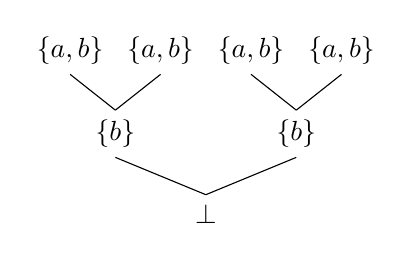
\begin{tikzpicture}[grow'=up]
   \Tree [.$\bot$  [.${\{b\}}$ ${\{a,b\}}$ ${\{\ol a,b\}}$ ] [.${\{ \ol b\}}$ ${\{a, \ol b\}}$ ${\{\ol a, \ol b\}}$ ] ]
   \end{tikzpicture}
   \caption{A resolution tree for Example \ref{exp:res1}.}
   \label{fig:resol1}
   \end{figure}
\end{examp}
%-------------------------------------------------------------------------
\section{DP-reduction}
\label{sec:dpr}

\begin{defi}\label{def:redctn}
A reduction is considered as a map $r: \Cls \ra \Cls$ such that for all $F \in \Cls$, $r(F)$ is satisfiability-equivalent to $F$. Using the reduction technique, unsatisfiability is resulted if $\bot \in r(F)$.
\end{defi}

An example of the reduction is unit resolution (or unit propagation) which is applied to a clause-set $F$ with at least one unit-clause (a clause with one literal). This technique is performed by setting the literal in unit-clause to its satisfying assignment. For example for clause $\set{x}$, we set the literal $x$ to true. If the reduction yields $\bot$, then $F$ is unsatisfiable. Else, if there are more unit-clauses, this step is continued until no unit-clause is left.

\begin{defi}\label{def:dpredc}
\cite{h9} The DP-reduction is the process of removing a variable $v \in \var(F)$ by taking all clauses having $v$ and replacing them by their resolvents that is:
\begin{displaymath}
\bmm{\dpi{v}(F)} := \set{C \in F : v \notin \var(C)} \cup \set{C \res D : C, D \in F \und C \cap \ol{D} = \set{v}} \in \Cls
\end{displaymath}
\end{defi}
Remarks:
  \begin{enumerate}
  \item If two clauses $C,D \in F$ have more than one clashes, by performing the DP-reduction on one of clashing variables both clauses are removed and we get nothing .
   \end{enumerate}
%%%%%%%%%%%%%%%%%%%%%%%%%%%%%%%%%%%%%%%%%%%%%%%%%%%%%%%%%%
\chapter{Hardness measures for Tseitin graph}
\label{cha:Hd-TseitinG}

\section{Hardness measures}
\label{sec:Hardnessmeasures}
The hardness is defined as a measure of complexity (the amount of effort needed to discover unsatisfiability) for a representation $F$ of a boolean function $f$ in SAT solving. Various hardness measures have been investigated in the literature and the relation between these measures is studied in \cite{h5,h18,h8}. In this proposal, two measures of the hardness are investigated. The first one is the tree-hardness which is related to the size of resolution proofs. The width-hardness is the second measure and is related to the width of clauses in resolution proofs. We start with defining these measures for unsatisfiable clause-sets and then, we extend the definitions to the satisfiable clause-sets. An overview of these two measure is given in \cite{h5,h18,?? }.

\subsection{Generalised unit-clause propagation}
\label{sec:rkred}

The unit resolution is explained in Section \ref{sec:dpr}. Another case of the reduction (Definition \ref{def:redctn}) is generalised unit-clause propagation introduced in \cite{h10} and denoted by $\rk_k$. 

\begin{defi}\label{def:rk}
\cite{h10} The maps $\rk_k: \Cls \ra \Cls$ for $k \in \NNZ$ are defined as follows (for $F \in \Cls$):
  \begin{eqnarray*}
  \rk_0(F) & := &
  \begin{cases}
  \set{\bot} & \text{if } \bot \in F\\ F & \text{otherwise}
  \end{cases}\\
  \rk_{k+1}(F) & := &
  \begin{cases}
  \rk_{k+1}(\pao x1 * F) & \text{if } \ex\, x \in \lit(F) : \rk_k(\pao x0 * F) = \set{\bot}\\ F & \text{otherwise}
  \end{cases}.
  \end{eqnarray*}
This technique removes some forced literals using forced assignments and discovers unsatisfiability if $\bot \in \rk_k(F)$.
\end{defi} 

Remarks:
\begin{enumerate}
  \item For $k=1$, the generalised unit-clause propagation eliminates all unit-clauses with assigning their satisfying assignment. Thus, $\rk_1$ is the unit-clause propagation.
  \item $\rk_2$ is called failed literal elimination and all clauses in $\rk_2$ have length at least $2$ (since all unit-clauses have already been removed).
  \item In each step $k$, if $\rk_k$ yields $\bot$ then the original clause-set $F$ is unsatisfiable while $F$ is satisfiable if $\top$ is obtained. In the latter case, the sequence of forced assignments eliminated until that level is a satisfying assignment for $F$.
  \item The map $\rk_k$ is well-defined since it does not depend on the choices of literals in each step. For example, in the process of obtaining  $\rk_1$ the final result does not change based on the order of choosing the unit literals. 
  \item For all clauses $C \in F$ if $\abs{C} > k$, then $\rk_k(F) = F$. This means that this technique is not complete since $\rk_k(F)$ can not discover the unsatisfiability of a clause-set $F$ if all clauses in $F$ have length at least $K+1$.
\end{enumerate}

\begin{examp}\label{exp:rk}
Using literals $a,b,c,d$, $\rk_k(F)$ for some examples is computed as follows:
  \begin{enumerate}
  \item $\rk_k(\set{\bot}) = \set{\bot}$ for $k \ge 0$ and $\rk_k(\top) = \top$ for $k \ge 0$.
  \item For $F := \set{\set{a},\set{b},\set{c},\set{d}}$: $\rk_0(F) = F$, $\rk_k(F) = \top$ for $k \ge 1$.
  \item For $F := \set{\set{a,b},\set{a,\ol{b}}, \set{\ol{a},b},\set{\ol{a},\ol{b}}}$: $\rk_k(F) = F$ for $k \le 1$, $\rk_k(F) = \set{\bot}$ for $k \ge 2$.
  \end{enumerate}
\end{examp}
%-----------------------------------------------------------------------
\subsection{Tree-hardness of clause-sets}
\label{sec:Hardnessunsat}

The concept of the hardness can be explained from two aspects. The first aspect is related to the complexity of resolution proofs and reviewed in \cite{h8, h18}. Following, we define the Horton-Strahler number as a measure of branching complexity for trees and we use it for resolution trees $T$.

\begin{defi}\label{def:hsn}
The Horton-Strahler number $\hts(T) \in \NNZ$ for each node of a resolution tree $T$ is the length of the shortest path from that node to the leaves. For the root of $T$,  $\hts(T)$ is the height of the tree.
\end{defi}
Remarks:
\begin{enumerate}
  \item To obtain $\hts(T)$, we start with leaves (axioms) whose Horton-Strahler number are defined as $\hts(T) := 0$. Then, for each inner node with two children $T_1, T_2$, we have two cases. If $\hts(T_1)= \hts(T_2)$, then $\hts(T) := \hts(T_1)+ 1$. Otherwise, $\hts(T) := \max(\hts(T_1),\hts(T_2))$.  For example, for all resolution trees $T:F \vdash \bot$ with $\hts(T) \leq 1$, every node is either a leaf or has a leaf as a child.
\end{enumerate}

\begin{defi}\label{def:hdhs}
\cite{h18} For an unsatisfiable clause-set $F$ there exist a resolution refutation $T:F \vdash \bot$ with the Horton-Strahler number (height) $\hts(T)$. The tree-hardness (or just hardness) for $F \in \Usat$ is defined as the minimum of $\hts(T)$ of all  $T:F \vdash \bot$ and denoted by $\hardness(F)$.
\end{defi}

From computational point of view, Definition \ref{def:hdhs} is not a practical method to obtain the hardness. Thus, there is another description using an algorithmic approach via generalised unit-clause propagation $\rk_k$. According to definition of $\rk_k(F)$ in \ref{def:rk}, the hardness is the minimum of $k \in \NNZ$ such that $\rk_k(F)$ yields $\bot$. This description is extended for satisfiable clause-sets in Definition \ref{def:hd-extended} based on \cite{h18, h8}.

\begin{defi}\label{def:hd-extended}
The hardness is a map that assigns a natural (and finite) number for a representation of a boolean function $f$ as a clause-set $F \in \Cls$ and is denoted by $\hardness : \Cls \rightarrow \NNZ$. To obtain the hardness of  $F$, there are three cases: if $F = \top$, then $\hardness(F) := 0$. Else if $F \in \Usat$, then $\hardness(F) := \min \set{k \in \NNZ : \rk_k(F)=\set{\bot}}$. Otherwise, $F \in \Sat \sm \set{\top}$ and $\hardness(F) := \max \set{ \hardness(\vp * F) : \vp * F \in \Usat }$.
\end{defi}

Remarks:
\begin{enumerate}
  \item Each satisfiable clause-set $F \in \Cls \sm \set{\top}$ can be converted to an unsatisfiable clause-set by applying a partial assignment $\vp$. For extending the hardness measure to a satisfiable clause-set, we should consider the worst case value of $\hardness$ for $\vp * F \in \Usat$ which is the maximum of $\hardness(\vp * F)$. The reason is that $\hardness(\vp * F) \leq \hardness(F)$ (the application of a partial assignment on $F$ do not increase the hardness) and one can easily find a $\vp$ such that $\bot \in \vp * F$ and $\hardness(\vp * F)=0$. For $\vp$ we only need to consider the minimal partial assignment which is $\vp_C : C \in \primec_0(F)$. For $F = \top$, since it is not convertible to an unsatisfiable clause-set, we assign the minimum of the hardness which is zero.  
  \item $\rk_k$ can not yield $\set{\bot}$ if all clauses in $F$ have length at least $k+1$.
\end{enumerate}

\begin{examp}\label{exp:harducls}
For $\set{\set{x,y},\set{x,\ol{y}},\set{\ol{x},y},\set{\ol{x},\ol{y}}}$ we have $r_1(F)=F, r_2(F)=r_2( \langle a \rightarrow 1 \rangle * F) = \{ \bot \}$(since $r_1( \langle a \rightarrow 0 \rangle * F)=r_1 (\{\{ b \}, \{ \ol b \}\}) = \{ \bot \}$). Thus, $\hardness(F) = 2$. In general, the hardness of full clause-sets are as $\hardness(A_n)=n$.
  
Following, $\hardness(F)$ for some more examples of unsatisfiable clause-sets $(F)$ are computed:
  \begin{enumerate}
  \item $\hardness(F) = 0$ if $\bot \in F$.
  \item $\hardness(\set{\set{a},\set{\ol{a}}}) = 1$.
  \item $\hardness(\set{\set{a},\set{\ol{a},b}, \set{\ol{b},c}, \set{\ol{c}}}) = 1$. 
  %In general, Horn clause-sets (whose clauses have at most one positive literal) have hardness one.
  \item $\hardness(\set{\set{a,\ol{b}},\set{\ol{a},b},\set{b,\ol{c}},\set{\ol{b},c},\set{a,b,c},\set{\ol{a},\ol{b},\ol{c}}}) = 2$.
  \end{enumerate}
\end{examp}

\begin{examp}\label{exp:hd-extd}
For $F = \set{\set{x, y} , \set{x,\ol y}} \in \Sat$ with $\primec_0(F) = \set{\set{x}}$,  $\hardness(F)= \max \set{ \hardness(\vp * F) : \vp =\pab{x \ra 0} }=\hardness(\set{\set{y},\set{\ol y}})=1$.
\end{examp}
%-----------------------------------------------------------------
\subsection{Width-hardness of clause-sets}
\label{sec:whdd}

Another measure for complexity of an unsatisfiable clause-set $F$ as in \cite{h18, h13} is the width-hardness (or asymmetric width) and indicated by $\whardness(F)$. 

As introduced in \cite{h19}:
\begin{defi}\label{def:kres}
Based on \cite{h33}, for a resolution proof $T: F \vdash C$ consider that each node (resolvent) in $T$ have at least one parent with length at most $k$. In this case, the resolvent is called $k$-resolvent. If every resolvent in $T$ is a $k$-resolvent, then $T:F \vdash C$ is called $k$-resolution and denoted by $F \vdash^k C$. For example, 1-resolution is the unit resolution.
\end{defi}
%If a $k$-resolution refutation exists then the unsatisfiability can be proved by the unit-preference strategy within k levels and vice versa \cite{h19}.

For each $F \in \Usat$ there exist a resolution refutation $T:F \vdash \bot$. The width-hardness of $F$ is the minimum of $k$ for all $k$-resolution trees $T:F \vdash \bot$. This definition is extended for a satisfiable clause-set $F$ in Definition \ref{def:whd-extended} by considering the worst case (maximum) of the width-hardness for the extended $F$ (that is $ \vp * F \in \Usat$) and $\whardness(\top):=0$.

\begin{defi}\label{def:whd-extended}
The width-hardness is a map denoted by $\whardness : \Cls \rightarrow \NNZ$ for a representation of a boolean function $f$ as a clause-set $F \in \Cls$. To obtain the width-hardness of  $F$, there are three cases: if $F = \top$, then $\whardness(F) := 0$. Else if $F \in \Usat$, then $\whardness(F) := \min \set{k \in \NNZ : F \vdash^k \bot}$. Otherwise, $F \in \Sat \sm \set{\top}$, and $\whardness(F) := \max \set{ \whardness(\vp * F) : \vp * F \in \Usat }$.
\end{defi}

For example if $\bot \in F$, then $F \vdash^0 \bot$ and $\whardness(F)=0$. Also if $\rk_1(F)=\set{\bot}$, then it is 1-resolution (unit resolution) and  $\whardness(F)=1$.
%-----------------------------------------------------------------
\section{Game characterisations of hardness measures}
\label{sec:game-pd}

overview in \cite{h18, h30,h31,?????}??????????

In \cite{h18}, a game is characterised to obtain $\hardness(F)$ or $\whardness(F)$ of a clause-set $F \in \Cls$ called the Prover-Delayer game (or just the hardness game). The game is performed between two players, Prover and Delayer. Delayer starts the game and two players play in turns. There is a partial assignment $\vp \in \Pass: \var(\vp) \sse \var(F)$ (initially empty) that is extended to $\vp'$ in each round by the two players. Therefore, in each round $k$ a new clause-set $F_k$ is obtained with $\hardness(F_k)$ (or $\whardness(F_k)$). The game ends once we reach certain conditions (for $\hardness(F)$ or $\whardness(F)$). First, we consider the game for $\hardness(F)$ and then we explain the game for $\whardness(F)$.

In the case of $\hardness(F)$, the goal is to set a strategy for both players in the Prover-Delayer game such that $\hardness(F)$ is achieved. Thus, we need to know that how $\hardness(F)$ is changed by extending $\vp$ with some variables $v \in \var(F)$. 

\begin{lem}\label{lem:hd-var}
\cite{h18} Consider a clause-set $F \in \Cls$ and $\hardness(F)$. If we assign a value $\ve \in \set{0,1}$ to a variable $v \in \var(F)$, then there are exactly two cases that can happen for $\hardness(F)$. The first case is $\hardness(\pab{x \ra \ve}*F)=\hardness(F)$ and $\hardness(\pab{x \ra \ol \ve}*F) \leq \hardness(F)$ and the second case is  $\hardness(\pab{x \ra \ve}*F)=\hardness(\pab{x \ra \ol \ve}*F)=\hardness(F)-1$. Thus, for all cases  $\hardness(\pab{x \ra \ve}*F) \leq \hardness(F)$.
\end{lem}

In this game, Delayer wants to maximize the $\hardness(F)$ for an unsatisfiable clause-set $F$. But since according to Lemma \ref{lem:hd-var} assigning one variable for $F$ (which yields $F'$) does not increase the hardness ($\hardness(F') \leq \hardness(F)$), Delayer must keep ($\hardness(F')$ unchanged. This is achieved by taking no action or just assigning those variables $x \in var(F): \hardness(\pab{x \ra \ve}*F)=\hardness(\pab{x \ra \ol \ve}*F = \hardness(F)$ (we call them as ineffective variables). 

On the other hand, Prover wants to minimize  $\hardness(F)$ and in each round, tries to choose a variable $x$ whose assigning reduces the hardness at most (like two or more points). Therefore, Delayer must prevent the case that Prover decreases the hardness more that one unit. This is achieved by assigning the other value for those variables. We call these variables $x \in var(F): \hardness(\pab{x \ra \ve}*F)=\hardness(F)$ and $\hardness(F)- \hardness(\pab{x \ra \ol \ve}*F) \geq 2$ as trouble makers. If Delayer succeeds in removing all trouble makers in each round, then Prover must decrease $\hardness(F)$ exactly one unit.
  
Since there is a finite number of variables in a clause-set, the game has a finite number of rounds (and therefore finite hardness for the clause-set). The game ends when we reach $\bot \in \vp * F $ (if $F$ is unsatisfiable) or $\vp * F=\top$ (if $F$ is satisfiable). In both cases, if $k$ rounds is played then $\hardness(F_k)=0$.

\begin{defi}\label{def:atomicmove}
For the clause-set $F$, the atomic move in the Prover-Delayer game for $\hardness(F)$ is the extension of the partial assignment  $\vp \in \Pass: \var(\vp) \sse \var(F)$.

In the case of Delayer, the atomic move is removing all trouble makers (by assigning a variable $v \in \var(F)$ such that the hardness remains unchanged) and then (when no trouble maker is left) assigning ineffective variables. In the case of Prover, the atomic move is assigning a variable $v \in \var(F)$ such that the hardness decreases exactly one unit.
\end{defi}

\begin{quest}
For  $x \in var(F): \hardness(\pab{x \ra \ve}*F)=\hardness(F)$ and $\hardness(F)- \hardness(\pab{x \ra \ol \ve}*F) =1$ in the case of Delayer, what is the optimal move?

Also, is the result of the game still the hardness of $F$ if Delayer does not assign all of ineffective variables in each round?
\end{quest}

\begin{lem}\label{lem:hdchg}
For $F \in \Usat$ by considering the strategy of both players based on Definition \ref{def:atomicmove}, $\hardness(F)$ in each round $k$ is as follows:
  \begin{eqnarray*}
  \hardness(F_k) & = &
  \begin{cases}
  \hardness(F_{k-1}) & \text{Delayer's turn }\\ \hardness(F_{k-1})-1 & \text{Prover's turn}
  \end{cases}
  \end{eqnarray*}
\end{lem}
\begin{prf}
XXX
\end{prf}

\begin{lem}\label{lem:gameres1}
Consider the Prover-Delayer game for an unsatisfiable clause-set $F$ with the goal of obtaining $\hardness(F)$. The hardness $\hardness(F)$ is exactly the number of rounds played by the Prover (or we can say that Prover gets a point in by performing an atomic move and the hardness of $F$ is equal to the Prover's points).

It should be mentioned that by considering performing exactly one atomic move in each round, the number of rounds $k$ is an even number. Thus, saying that the hardness equals to $k / 2$ is equivalent to the above statement.
\end{lem}
\begin{prf}
For $F \in \Usat$, the game ends once we get $\bot \in \vp * F $. Thus if the game is played in $n$ rounds, then $\hardness(F_n)=0$. On the other hand, according to Lemma \ref{lem:hdchg} we know that in each round played by Prover the $\hardness(F)$ is decreased exactly by one unit and in the other rounds, it remains unchanged. Therefore, $\hardness(F)$ is the number of rounds played by the Prover.
\end{prf}

\begin{lem}\label{lem:gameres2}
Consider the Prover-Delayer game for an arbitrary clause-set $F \in \Cls$ with the goal of obtaining $\hardness(F)$. If $F \in \Usat$, then the hardness $\hardness(F)$ is exactly the number of Prover's atomic moves. Else, $F \in \Sat$ and $\hardness(F)=0$.
\end{lem}
\begin{prf}
For $F \in \Usat$, see Lemma \ref{lem:gameres1}. For $F \in \Sat$, the game ends when we reach $\vp * F=\top$. Thus $\vp$ is a satisfying assignment for $F$ and $\hardness(F)=0$
\end{prf}

\begin{lem}\label{lem:game1}
The game is well-defined (it does not depend on choices).
\end{lem}
\begin{prf}
According to Definition \ref{def:atomicmove} the Delayer first assigns all variables that are trouble maker to prevent the case that the hardness reduction is more than one units. Then it assigns all ineffective variables in each round. Thus, the order of choosing variables by Delayer in each case does not affect the result. For Prover, it chooses one of the variables (that assigning them reduces the hardness exactly one unit) in each round and chooses the rest of them in next rounds (since Delayer would not assign them). Thus, the order of choosing variables by Prover does not affect the result of game.
\end{prf}

\begin{examp}\label{exp:gamehd}
Consider a clause-set $F=\set{\set{a,b},\set{\ol a,b},\set{a,\ol b},\set{\ol a,\ol b},\set{c},\set{\ol c}} \in \Usat$. Then, ?????

And for $F=\set{\set{a,\ol{b}},\set{\ol{a},b},\set{b,\ol{c}},\set{\ol{b},c},\set{a,b,c},\set{\ol{a},\ol{b},\ol{c}}} \in \Usat$, ???
\end{examp}
%------------------------------

The for $\whardness(F)$???

\begin{defi}\label{def:atomic-move}
For the clause-set $F$, the atomic move in the Prover-Delayer game for $\whardness(F)$ is ???????????
In the case of Delayer, the atomic move is???

In the case of Prover, the atomic move is ????
\end{defi}
%%%%%%%%%%%%%%%%%%%%%%%%%%%%%%%%%%%%%%%%%%%%%%%%%%%%%%%%%%
%\chapter{Hardness measures for Tseitin graph}
%\label{cha:hdgame}

\section{XOR representation}
\label{sec:XOR representation}
For representing a boolean function $f$ we defined CNF-clause-sets in Section \ref{sec:Clause-sets}. Here, another representation of $f$ is introduced (called XOR-representation) which is used for extending the hardness game for graphs based on \cite{h8,h23}. An XOR-clause-set for $f$ is the interpretation of a clause-set $F \in \Cls$ as a system of XOR-constraints whose clauses $C$ are parity equation for $v \in \var(C)$. 
as in??????????????
\begin{defi}\label{def:xor-const} 
An XOR-constraint (or parity constraint) is a boolean function (parity function) $f$ in the form of $x_1 \oplus \dots \oplus x_n = \ve$ that $x_1, \dots, x_n \in \Lit$ and $\ve \in \set{0,1}$.
\end{defi}

Remarks:
\begin{enumerate}
    \item $x_1 \oplus \dots \oplus x_n = y$ is equivalent to $x_1 \oplus \dots \oplus x_n \oplus y = 0$
    \item $x \oplus x = 0$, $x \oplus \ol{x} = 1$, $0 \oplus x = x$, $1 \oplus x = \ol{x}$.
    \item Two XOR-constraints $f_1, f_2$ are equivalent iff $\var(f_1) = \var(f_2)$ and both have the same parity for literals.
\end{enumerate}

\begin{defi}\label{def:xor-cls}
Based on \cite{h8}, an XOR-clause $C \in \Cl$ with literal $x \in \Lit$ is an XOR-constraint with $\oplus_{x \in C} = 0$. Thus, two XOR-clauses $C, D$ are equivalent iff $\var(C) = \var(D)$ and both with the same parity. In an XOR-clause, there is no repetitive literals since $x \oplus x = 0$. In the case of clashing literals, we remove them using the laws $x \oplus \ol{x} = 1$ and $1 \oplus y = \ol{y}$ (since according to the definition, clashing literals are not allowed in clauses).

An XOR-clause-set is a clause-set $F \in \Cls$ whose clauses $C$ are interpreted as an XOR-clause.  
\end{defi} 

Remarks:
\begin{enumerate}
  \item The operation of a partial assignment $\vp \in \Pass$ to XOR-clause-sets is defined as the same definition for CNF-clause-sets.
  \item An XOR-clause-set $F$ is satisfiable if there exist a partial assignment $\vp$ such that $\var(\vp) \supseteq \var(F)$ and for every $C \in F$ the number of $x \in C$ with $\vp(x) = 1$ is even (that satisfies the equation  $\oplus_{x \in C} = 0$).
\end{enumerate}

The satisfiability of a CNF-clause-set is investigated using the resolution operation. Here, for investigating whether an XOR-clause-set is satisfiable or not, an operation is defined based on \cite{h8,h23} which is called an XOR-sum over clauses of $F$.

\begin{defi}\label{def:xor-sum}
\cite{h8} The XOR-sum over clauses of $F$ denoted by $\oplus F \in \Cl$ is applied to two XOR-clauses and produces a new clause or the result is inconsistent. The operation is performed as follows. If there are four literals as $x,\ol{x},y,\ol{y}$ for $x \ne y$, the XOR-sum of them is as $x \oplus \ol{x} = 1$ and $y \oplus \ol{y} = 1$. Thus, $1 \oplus 1 = 0$ and they are removed. If no clash remains, then the result is obtained as a clause $E \in \Cl$. Else if there is just one clash for literals $x, \ol{x}$ with at least one other literal $y$, then $x \oplus \ol{x} = 1$ and $1 \oplus y=\ol{y}$ and a new clause $E \in \Cl$ is obtained. Otherwise, if two literals $x, \ol{x}$ remains, then $\oplus F$ is called inconsistent. An XOR-clause-set $F \in \Cls$ is unsatisfiable if and only if there is $F' \sse F$ such that $\oplus F'$ is inconsistent.
\end{defi} 

\begin{examp}\label{exp:xorcls}
The satisfiability of the following XOR-clause-sets $F$ are investigated using the XOR-sum over clauses of $F$.
  \begin{enumerate}
  \item For $F=\top$, $ \oplus(F)= \oplus(\set{\bot})=\bot$ and $F$ is satisfiable.
  \item For $F=\set{\set{a,b},\set{b,c,\ol d}}$, $ \oplus(F) = \set{a,c,\ol d}$ and $F$ is satisfiable.
  \item For $F=\set{\set{a,b,c},\set{a, \ol b, \ol c}}$, $ \oplus(F) = \bot$ and $F$ is satisfiable.  
  \item  For $F=\set{\set{a,b},\set{a, \ol b},\set{c,d}}$, $\oplus (F)$ is inconsistent and $F$is unsatisfiable.
  \end{enumerate}
\end{examp}

For each XOR-clause-set $F$ there is a unique equivalent CNF-clause-set $F'$ (without auxiliary variables). To obtain this equivalent CNF-clause-set, a translation is defined and indicated by $X_0(F)$. This translation, converts each clause of $F$ to a set of full clauses in CNF-representation and then $F'$ is the union of these sets. If $F$ has long clauses, then obtaining $X_0(F)$ is not practical.

\begin{defi}\label{def:x0tr}
\cite{h8} The $X_0$ translation is a map $X_0: \Cls \ra \Cls$ where the input is an XOR-clause-set and the output is a  CNF-clause-set. Consider an XOR-clause $C \in F$, the $X_0$ translation of this clause is defined as the set of prime implicates of the boolean function for $C$ (without auxiliary variables) and indicated by $X_0(C)=\primec_0(x_1 \oplus \dots \oplus x_n = 0)$. The translation $X_0(C)$ contains all the full clauses over the set of variables in $C$ whose parity are different from the parity of $C$. Thus, $\abs{X_0(C)}=2^{\var(C)-1}$. Finally, the CNF-clause-set is obtained by $X_0(F) := \bc_{C \in F} X_0(C)$.
\end{defi} 

\begin{examp}\label{exp:X0}
For $F=\set{\set{a,\ol b}}$, $X_0(F)= \set{\set{a,b},\set{\ol a,\ol b}}$ and for $F=\set{\set{a},\set{b,c}}$, $X_0(F)=\set{\set{\ol a},\set{\ol a, b}, \set{a, \ol b}}$.
\end{examp}
%-----------------------------------------------------------------
\subsection{Tseitin graph}
\label{sec:Tseitin graph}

Based on \cite{h34,h8} ???????

For extending the hardness game for graphs, first we need to describe Tseitin graph and Tseitin clause-set. A simple graph is a pair $G = (V,E)$ where $V$ is the set of vertices and $E$ is the set of edges. If we consider the graph as a triple $G = (V,E,\eta)$ such that $V$ is the set of vertices, $E$ is the set of edge-labels and $\eta: E \ra \set{e \sse V : 1 \le \abs{e} \le 2}$, we can describe parallel edges and loops. 

Consider a connected graph $G=(V,E,\eta)$ without loop. First, we label each edge with a distinct literal $x \in E$. Then, if we assign a charge $\rho$ to each vertex such that $\rho: V \ra \set{0,1}$, we obtain a unique XOR-clause-set corresponded to $G$. In this case, each vertex $w \in V$ is specified as an XOR-clause $C \in \Cl$ such that $\oplus_{x \in E, w \in \eta(x)} \; x = \rho(w)$. Then, the XOR-clause-set for $G$ is obtained by $T_0(G,\rho) := \set{C_w : w \in V} \in \Cls$. 

\begin{lem}\label{lem:chgvar}
Suppose that $T_0(G,\rho)$ is an XOR-clause-set for a graph $G=(V,E,\eta)$ without loop. We define $\Phi$ as an XOR-constraint for charges of vertices that is $\oplus_{w \in V} \rho(w) = \ve$ and $\ve \in \set{0,1}$. By assigning a value to all edges $x \in E$, we obtain $\rho(w)$ of all vertices and then, the value of $\ve$ in $\Phi$. In this case, if we change the value of an edge $x$, then $\rho(w)$ for each endpoint of $x$ must be changed to keep $\Phi$ unchanged.
\end{lem}
\begin{prf}
According to the definition, each vertex $w$ of $G$ is an XOR-clause with $\rho(w)$ such that  $\oplus_{x \in E, w \in \eta(x)} \; x = \rho(w)$ ($\rho$ is the parity). Since each literal corresponds to an edge connected to two vertices $w_1, w_2$, changing the value of a literal $x$ will change the parity $\rho(w)$ for equation of $w_1, w_2$. XXX
\end{prf}

For a graph such as Lemma \ref{lem:chgvar} with $\Phi$, if $\ve=0$ then we need to investigate the satisfiability of each XOR-clause to determine whether $T_0(G,\rho)$ is satisfiable or not. Else if $\ve=1$, then $T_0(G,\rho)$ is unsatisfiable. The reason is as follows. If $\ve=1$ in $\Phi$, there is at least one vertex $w$ (XOR-clause $C$) with $ \rho(w) =1$ and according to the definitions in Section \ref{sec:XOR representation}, an XOR-clause $C$ is satisfiable if $\oplus_{x \in C} = 0$. Thus, $\oplus_{x \in C} = \rho(w) \not =0$ and $T_0(G,\rho)$ is unsatisfiable.

A graph $G$ as explained in Lemma \ref{lem:chgvar} with $\ve=1$ in $\Phi$, is called a Tseitin graph. The equivalent CNF-clause-set of $G$ is obtained by $X_0$ translation of $T_0(G,\rho)$ and indicated by $T(G,\rho) := X_0(T_0(G,\rho))$. The clause-set $T(G,\rho) \in \Usat$ is called the Tseitin clause-set of $G$.
%----------------------------------------------
\section{Application of game characterisation for hardness of Tseitin graph}
\label{sec:appgame}

\subsection{Game-tree}
\label{sec:Game-tree}

For each Tseitin clause-set $F$ corresponding to a Tseitin graph $G$, there exist a unique tree called game-tree such that shows all possible atomic moves for Prover and Delayer. The tree is upside down with even number of levels and the root of the tree is $F$. Each node of the game-tree (except leaves) corresponds to a clause-set $F'$ ($ \bot \not \in F'$) whose variable is at most one unit less that the upper-level nodes. The children of each node are the all possible atomic moves in that round. Each path from root must end in a leaf since the edges of graph (which correspond to the maximum of atomic moves of Prover) are finite and the leaves correspond to $\bot$. ????????The hardness of $F$ is achieved by assigning a number to each node (starting from leaves) and obtaining the number of the root.

To obtain the harness, first we assign a number to each leaf that corresponds to the scores of Prover (the number of Prover's atomic moves) through the path to that leaf. Since the last round of game is always played by Prover, we assign the minimum number of leaves to their parents (upper-level nodes). Then, we consider the upper level which is played by Delayer and therefore, we assign the maximum number of nodes for their parents. This process is continued until we get the root and and we assign the maximum number of root's children to the root (since the first round is played by delayer). Finally, the hardness of $F$ corresponds to the number of the root.

\begin{lem}\label{lem:game2}
For each arbitrary clause-set $F \in \Usat$, the game-tree is unique.
\end{lem}
\begin{prf}
??????????
\end{prf}

\begin{examp}\label{exp:gg1}
Fig \ref{fig:gg1} shows the game-tree for graph $K_3$. The children of each node are all possible moves (whether the move is optimal or not) in hardness game for $K_3$. Here, $\ve $ shows the empty move (or when delayer decides to do nothing) and $\bot$ shows the end of game. We start from leaves by counting the number of prover's moves until that leaf and assign this number to that leaf. 
   \begin{figure}
   \begin{center}
   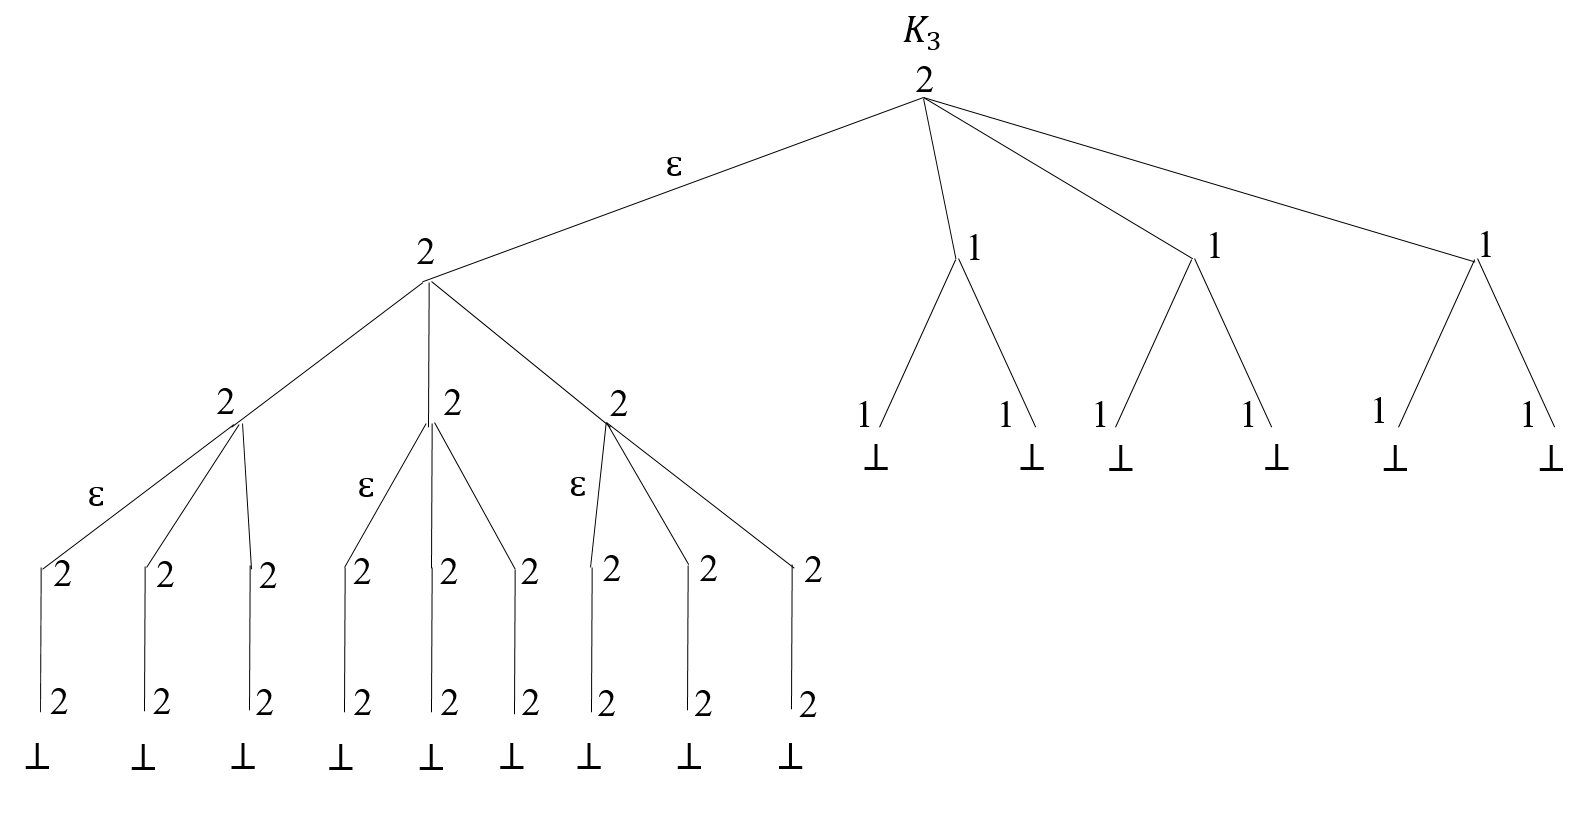
\includegraphics[scale =0.45]{gg1.png}
   \caption{The game-tree for $K_3$.}
   \label{fig:gg1}
   \end{center}
   \end{figure}
\end{examp}
%----------------------------------------------
\subsection{Game characterisations for Tseitin graph}
\label{sec:hd-game-graph}

Here, ???

\begin{defi}\label{def:bridge}
Consider a Tseitin graph $G$ as explained in Section \ref{sec:Tseitin graph}. If there is an edge $e \in E$ whose deletion increases the number of connected components of $G$, then $e$ is called a bridge.
\end{defi} 

Consider an unsatisfiable Tseitin clause-set $T(G,\rho)$. ??????????

\begin{lem}\label{lem:game3}
In a Tseitin graph $G$ if we remove an edge $e \in E$, then $\rho(w)$ of endpoints will change. 
\end{lem}
\begin{prf}
According to the definition of a Tseitin graph $G$, the XOR-clause-set $T_0(G,\rho)$ is unsatisfiable since $\ve=1$ for $\Phi$. Thus based on lemma xxx, too keep $\ve=1$ unchanged, if we remove any edge by assigning a value, then the equation of endpoints must be changed
\end{prf}

\begin{defi}\label{def:atomicmovegraph}
For ?????????, the atomic move in the Prover-Delayer game for $\hardness(F)$ is ??????????

In the case of Delayer, the atomic move is removing ????????
In the case of Prover, the atomic move is ?????????????
\end{defi}

\begin{lem}\label{lem:Tseitingame1}
The game is well-defined (it does not depend on choices). 
\end{lem}
\begin{prf}
According to ???????? the Delayer assigns all variables that are trouble maker (the variables that Prover can assign a value to them such that the hardness decreases more that one units) to prevent the case that the hardness reduction is more than one units. Thus, the result of the game does not depend to the order of choosing variables in each round
\end{prf}

\begin{quest}\label{que:game}
???? for hd and whd
\end{quest}
%%%%%%%%%%%%%%%%%%%%%%%%%%%%%%%%%%%%%%%%%%%%%%%%%%%%%%%%%%
\chapter{Structure of minimally unsatisfiable clause-sets}
\label{cha:mucls}

\section{Background}
\label{sec:basicdef}

One of the main class of unsatisfiable clause-sets are minimally unsatisfiable clause-sets which is referred as the building block for understanding unsatisfiability in \cite{h9}. So, understanding the concept of minimally unsatisfiable clause-sets and investigating their properties and subclasses are important. An overview of these clause-sets are presented in \cite{h9, h25,h29}. An interesting measure for the complexity of clause-sets and particularly minimally unsatisfiable clause-sets is deficiency. In this section we use this measure for classification of minimally unsatisfiable clause-sets which is already investigated in \cite{h9, h25,h26,h24, h27}.

\begin{defi}\label{def:mu}
A clause-set $F \in \Usat$ is minimally unsatisfiable if by removing any arbitrary clause $C \in F$, the clause-set $F \sm \set{C}$ becomes satisfiable. The set of all minimally unsatisfiable clause-sets is indicated by $\Musat \in \Usat$.
\end{defi}
Remarks:
  \begin{enumerate}
  \item The complexity of the problem $\Musat \in \Usat$ is $D^P$-complete (by Theorem 11.1.1 in \cite{h25}).
  \item All full clause-sets $ A_n$ are in $\Musati{}$.
  \end{enumerate}

\begin{defi}\label{def:deficiency}
The deficiency for a clause-set $F \in \Cls$ is defined as the difference between the number of clauses and the number of variables and indicated by $\delta \in \ZZ: \delta(F)= c(F) - n(F)$.
\end{defi}
Remarks:
  \begin{enumerate}
  \item In this report, the minimally unsatisfiable clause-sets with deficiency $k \in \ZZ$ are indicated by $\Musati{\delta=k}$.
  \item The complexity of the problem $\Musati{\delta=k}$ for fixed $k$ is $P$ (by Theorem 11.2.1 in \cite{h25}).
  \item All $F \in \Musati{\delta=k}$ have $k \ge 1$ (by Theorem 8 in \cite{h32}).
  \end{enumerate}

\begin{defi}\label{def:degree}
For a clause-set $F \in \Cls$ the literal degree for a literal $x \in \lit(F)$ is the number of the literal occurrence and denoted by $\ldeg_F(x) \in \NNZ$. The variable degree for a variable $v \in \var(F)$ is defined as $\vdeg_F(v) := \ldeg_F(v) + \ldeg_F(-v) \in \NNZ$. Finally, the minimum variable degree (or min-var-deg) is defined as the minimum of variable degree for all variable in $F$ and indicated by $\minvdeg(F) \in \NN$.
\end{defi}
Remarks:
  \begin{enumerate}
  \item It is obvious that $\vdeg_F(v) \le 2 \delta(F)$ and thus for $n(F) >0$, $\minvdeg(F) \le 2 \delta(F)$. A sharper upper bound for $\minvdeg(F)$ is given in Theorem 9.10 of \cite{h9}.
  \item All full clauses $A_n$ have deficiency $2^n - n$ and if $n \ge 1$, then  $\minvdeg(A_n) =2^n$.
  \item In \cite{h9}, the problem of finding the min-var-deg for minimally unsatisfiable clause-sets with fixed deficiency is indicated by $\minnonmer(k) $ (that is $\minnonmer(k)  :=  \minvdeg(\Musati{\delta=k}) \in \NN$) and an improved upper bound/ lower bound for $\minnonmer(k) $ is given.
    \end{enumerate}
    
\begin{defi}\label{def:singvar}
By \cite{h29}, for a variable $v \in \var(F)$ if $\min(\ldeg_F(v) ,\ldeg_F(-v))=1$ and is not pure, then it is called a singular variable. If a clause-set $F$ does not have any singular variable, it is called nonsingular. An m-singular variable is a singular variable with $\vdeg_F(v)=m+1$, $m \in \NN$.
\end{defi}
Remarks:
  \begin{enumerate}
  \item The set of nonsingular minimally unsatisfiable clause-sets $F \in \Musat$ are indicated by $\Musat' \in \Musat$. Thus, if $F \in \Musat'$, then all variables in $F$ are occurred at least twice positively and at least twice negatively.
  \item A non-1-singular variable is a variable which $m$-singular for some $m \ge 2$.
   \end{enumerate}
 
\begin{defi}\label{def:splitting}
Consider a variable $v \in \var(F)$. Splitting of $F$ on $v$ is the process of obtaining two clause-set $F_0,F_1$ as  $F_0:=\pao v0 * F$ and $F_1:=\pao v1 * F$.
\end{defi}
Remarks:
  \begin{enumerate}
  \item A clause-set $F$ in $\Musati{\delta=k}$, splitting may leads to produce two minimally unsatisfiable clause-sets $F_0,F_1$ but generally we can not say this for sure unless more information are provided (see Section \ref{???}). 
  \item If a clause-set $F$ is in $\Musatnsi{\delta=k}$ and also after splitting on a variable the clause-sets $F_0,F_1$ are minimally unsatisfiable with deficiency $k_0, k_1$, then we have $k_0, k_1 < k$ (by Theorem 2 in \cite{h24}).
  \item For $F \in \Musat$, the application of splitting for $\delta=1$ and $\delta=2$ are investigated in Sections \ref{} and \ref{}. ?????????
  \end{enumerate}
%-----------------------------------------------------------------------------
\section{Autarkies}
\label{sec:autrk}

\begin{defi}\label{def:autarky}
For a clause-set $F$ a partial assignment $\vp \in \Pass$ is called an autarky if $\fa\, C \in F : \vp * \set{C} \in \set{\set{C}, \top}$. That is whenever a clause is touched by a partial assignment $\vp$, then $\vp$ satisfies it.
\end{defi}
Remarks:
  \begin{enumerate}
  \item If $\vp$ is an autarky for a clause-set $F$, then the application of $\vp *F$ is sat-equivalent for $F$. 
  \item All satisfying assignment for $F$ are autarky.
  \item The empty partial assignment $\epa$ is an autarky for every $F \in \Cls$ and more generally all $\varphi \in \Pass$ with $\var(\varphi) \cap \var(F) = \emptyset$ are autarkies for $F$. 
  \item An autarky $\vp$ for $F$ is called trivial if $\var(f) \cap \var(\vp) = \es$. Else, it is called non-trivial autarky.
  \item A clause-set with no non-trivial autarky is called a lean clause-set. The set of all lean clause-sets is denoted by $\Lean \subset \Usat \addcup \set{\top}$. An overview on autarkies and lean clause-sets are given in \cite{h28, h25}. 
  \end{enumerate}
  
\begin{defi}\label{def:autarky-redc}
If $\vp \in \Pass$ is a non-trivial autarky for a clause-set $F$, then $\vp *F$ is called autarky reduction for $F$ (and is sat-equivalent to $F$).
\end{defi} 
Remarks:
  \begin{enumerate}
  \item If we apply all possible autarky reduction for a clause-set $F$, then we get lean kenrel of $F$ (Section 11.8.3 in \cite{h25} provides more details of lean kernel). The lean kernel is the largest lean sub-clause-set of $F$.
  \item Another equivalent description for lean clause-sets according to \cite{h28} is that if $F \in \Lean \sm \top$ then every clause $C \in F$ is used in at least one resolution refutation for $F$. Thus, the lean kernel of $F$ is the set of all clauses from $F$ that can be used in at least one resolution refutation for $F$ (by Theorem 11.8.1 in \cite{h25}).
  \item The autarky reduction is obtained a polynomial time, but finding the autarky in polynomial time is still an open question (\cite{h9} in Section 10.1 discusses whether the autarky can be found in polynomial time).
  \end{enumerate}
%-----------------------------------------------------------------------------
\section{Hitting clause-sets}
\label{sec:hit}

\begin{defi}\label{def:hit-cls}
A clause-set $F \in \Cls $ is called a hitting clause-set iff all clauses $C,D \in F$, $C \not = D$ have at least one clash. The set of all hitting clause-sets is indicated by $\Clash \in \Cls$.
\end{defi}
Remarks:
  \begin{enumerate}
  \item The set of all unsatisfiable hitting clause-sets is indicated by $\Uclash := \Usat \cap \Clash$. The set of all nonsingular unsatisfiable hitting clause-sets is denoted by $\Uclash'$ ($\Uclash' \subset \Uclash$).
  \item If $F \in \Uclash$, then every clause $C \in F$ is a satisfying assignment (as a partial assignment) for $F \sm \set{C}$.
  \item If $F \in \Musat$ then removing any clause $C \in F$ make $F \sm \set{C}$ satisfiable. On the other hand, if $F \in \Uclash$ then every $C \in F$ is a satisfying assignment for $F \sm \set{C}$. Thus, $\Uclash \subset \Musat$. \cite{h26} gives overview of unsatisfiable hitting clause-set.
  \item For all full clauses $A_n$ we have $A_n \in \Uclash$.
  \end{enumerate}

 \begin{defi}\label{def:nhit-cls}
A clause-set $F \in \Cls $ is called a nearly-hitting clause-set iff for all clauses $C,D \in F$, $C \not = D$ either $\var(C) \cap \var(D) = \es$ or $C,D$ have at least one clash. The set of all nearly-hitting clause-sets is denoted by $\Nclash \subset \Cls$.
\end{defi}
Remarks:
  \begin{enumerate}
  \item If $F \in \Nclash$ then every $C \in F$, as partial assignment, is an autarky for $F \sm \set{C}$.
  \end{enumerate}
  
\begin{quest}\label{ques:nhit-sat}
The complexity of SAT-decision for nearly-hitting clause-sets is open (also in the boolean case).
\end{quest}
   
 %-----------------------------------------------------------------------------              
\section{Saturated minimally unsatisfiable clause-sets}
\label{sec:smu}

\begin{defi}\label{def:smu}
A clause set $F \in \Cls$ is called saturated minimally unsatisfiable iff $f \in \Musat $ and by replacing any $C \in F$ by any super-clause $C' \supset C$, the result clause-set is satisfiable. The set of all saturated minimally unsatisfiable clause-sets is denoted $\Smusat \subset \Musat$.
\end{defi}
Remarks:
  \begin{enumerate}
  \item The set of all nonsingular saturated minimally unsatisfiable clause-sets is indicated by $\Smusatns \subset \Smusat$.
  \item For all clause-sets $F \in \Cls$, if $F \in \Uclash$ then $ F \in \Smusat$ ,i.e. $\Uclash \subset \Smusat$ (by Lemma 2 in \cite{h29}). 
  \item The properties of clause-set in $\Smusatnsi{\delta=1}, \Smusatnsi{\delta=2}$ are investigated in Sections \ref{} , \ref{}.
  \item For every $F \in \Musat$ there is a saturation $F' \in \Smusat$. A saturated clause-set  $F'$ for $F$ is obtained using an operation defined in Definition \ref{def:smu-opr}.
  \end{enumerate}

\begin{defi}\label{def:smu-opr}
\cite{h29} For every $F \in \Musat$ a saturation $F' \in \Smusat$ is obtained by iterated application of the operation $\saturate(F,C,x)$ as follows where $C \in F$, $x \in \lit(F)$ and $\var(x) \not \in \var(C)$:
  \begin{displaymath}
    \saturate(F,C,x) := (F \sm \set{C}) \cup (C \addcup \set{x}) \in \Cls
  \end{displaymath}
If in iteration $m$ there is no literal in $F$ fulfilling the condition $\var(x) \not \in \var(C)$ for all clauses of $F$, then $F' =\saturate(F_m,C_m,x_m) \in \Smusat$. 
\end{defi}
Remarks:
  \begin{enumerate}
  \item If $F' \in \Smusat$ is a saturation for $F \in \Musat$, then we have $n(F')=n(F)$, $c(F')=c(F)$ and $\delta(F')=\delta(F)$.
  \item If $C \in F$ and $\var(C) = \var(F)$ then no literal can be added to $C$ to make $F$ saturated and all full clauses $A_n$ are in $\Smusat$.
  \end{enumerate} 
  
\begin{examp}\label{exp:smu-exp}
  For $F = \set{\set{a,b},\set{\ol{a}},\set{\ol{b}}} \in \Musat \sm \Smusat$ using the Definition \ref{def:smu-opr} we can have $F'=\set{\set{a,b},\set{\ol{a},b},\set{\ol{b}}} \in \Smusat$ or $F'=\set{\set{a,b},\set{\ol{a}},\set{a,\ol{b}}} \in \Smusat$.
\end{examp}
%-----------------------------------------------------------------------------
\section{Reduction/ extension of minimally unsatisfiable clause-sets}
\label{sec:r-e}

To understand the structure of minimally unsatisfiable clause-sets and finding the isomorphism types of $\Musati{\delta=k}$ some types of reduction/ extension of clause-sets are reviewed in this section according to \cite{h9,h29}.

\subsection{Singular reduction/ extension}
\label{sec:sing-re} 

\begin{defi}\label{def:singularDP}
Consider DP-reduction in Definition \ref{def:dpredc}. If the DP-reduction is performed for a singular variable, then it is called the singular DP-reduction and the set of all nonsingular clause-sets obtainable from $F$ by singular DP-reduction denoted by $sDP(F)$. 
\end{defi}
Remarks:
  \begin{enumerate}
  \item Base on Lemma 5.3 in \cite{h9}, if a clause-set $F$ is minimally unsatisfiable then after performing the singular DP-reduction, the result clause-set $F'$ is also minimally unsatisfiable. This is also true when $F$ is in $\Smusat$ or $\Uclash$.   Further more, the singular DP-reduction does not change the deficiency of $F$ since $c(F)$ and $n(F)$ both decreased by one (an overview of DP-reduction for minimally unsatisfiable clause-sets is presented in \cite{h29}).
  \item For $F \in \Musat$, the application of $sDP$ for $\delta=1$ and $\delta=2$ are investigated in Sections \ref{} and \ref{}. ?????????
  \end{enumerate}
  
\begin{lem}\label{lem:sDP-infl}
For a clause-set $F \in \Musati{\delta=k}$:
  \begin{enumerate}
  \item If $k=1$ then an iterated application of singular DP-reduction leads to $\set{\bot}$ (that is $sDP(F)=\set{\bot}$).
  \item If $k \ge 2$, then an iterated application of singular DP-reduction leads to a clause-set in $\Musatnsi{\delta=k}$ (by Lemma 1 in \cite{h24}).
  \end{enumerate}
\end{lem} 

\begin{defi}\label{def:singularextn}
By \cite{h9} for a clause-set $F \in\Cls$ and a variable $v \not \in \var(F)$, the singular extension is defined as the reverse direction of singular DP-reduction. Also, a singular m-extension of $F$ to $F'$ with $v$ is as follows:
  \begin{displaymath}
    F' := (F \sm \set{D_1,\dots,D_m}) \addcup \set{C', D_1'',\dots,D_m''}.
  \end{displaymath}
where $\var(x)=v$, $D_1, \dots, D_m \in F$ are different clauses, $C \sse \bca_{i=1}^m D_i$ and $D_i' \in \Cl$ for $i \in \tb 1m$ with $(D_i \sm C) \sse D_i' \sse D_i$. Also, $C' := C \addcup \set{x}$, and $D_i'' := D_i' \addcup \set{\ol{x}}$ for $i \in \tb 1m$. Then, $F'$ is obtained from $F$ by adding $C'$ and replacing the $D_i$ with $D_i''$.
\end{defi}
Remarks:
  \begin{enumerate}
  \item Consider an $m$-extension $F'$ of $F$. Then, $F \in \Musat \Lra G \in \Musat$ (by Lemma 5.9 in \cite{h9}).
  \item The singular m-extension of $F$ does not change the deficiency of $F$. But, number of clauses (and variables) is increased by one.
  \end{enumerate}
  
\begin{defi}\label{def:unit-ext}
By \cite{h9} for a clause-set $F \in \Cls$, a full singular unit-extension $F' \in \Cls$ is obtained as follows: First, consider a literal $x:\var(x) \notin \var(F)$. Then, $F' := \set{\set{x}} \addcup \set{C \addcup \set{\ol{x}} : C \in F}$. Thus, $F' $ has a unit clause $\set{x}$ and all clauses of $F$ with literal $\ol{x}$ added to them.
\end{defi}
Remarks:
  \begin{enumerate}
  \item Consider $F'$ as the full singular unit-extension of $F$, if $F \in \Musati{\delta=k} $ the  $F' \in \Musati{\delta=k} $. This is also true about $F \in \Smusati{\delta=k}$. (by Lemma 5.17 in \cite{h9}).
  \end{enumerate}
%-----------------------------------------------------------------------------
\subsection{Full subsumption resolution/ extension}
\label{sec:fsr-e}  
    
\begin{defi}\label{def:fsr}
\cite{h9} The strict full subsumption resolution is the reduction of $F \in \Cls$ to $F'$ as follows and indicated by $F \tsubres F'$. To obtain $F'$, consider a clause $R \in F'$ (the resolvent) and a literal $x \in \var(F'):\var(x) \notin R$ ($x, \ol{x}$ the resolution literals). Then if $C := R \addcup \set{x}$ and $D := R \addcup \set{\ol{x}}$ (the parent clauses), then we have $F = (F' \sm \set{R}) \addcup \set{C,D}$.

$F \tsubresk{k} F'$ for $k \in \NNZ$ shows application of exactly $k$ steps of strict full subsumption resolution. If the resolution variable is allowed to vanish, then it is called Full subsumption resolution.
\end{defi}

    
\begin{defi}\label{def:fse}
Based on \cite{h9} the strict full subsumption extension in the reverse direction of the strict full subsumption resolution. Thus by considering the parameters in Definition \ref{def:fsr} for $F, F'$ and $F \tsubres F'$, the clause $R$ is expanded to $C = R \addcup \set{x}$, $D = R \addcup \set{\ol{x}}$ and we say $F$ is obtained from $F'$ by strict full subsumption extension.
\end{defi}
Remarks:
  \begin{enumerate}
  \item If $F \in \Musat $ then $ F' \in \Musat$ and also if $F \in \Smusat$ we have $ F' \in \Smusat$ while if $ F' \in \Smusat$ then $F \in \Musat $ ( by Lemma 6.5 in \cite{h9}).
  \item 
  \end{enumerate}
    

%-----------------------------------------------------------------------------
\section{Classification of minimally unsatisfiable clause-sets}
\label{sec:c-mucls}

Considering definitions and tools given in previous sections, minimally unsatisfiable clause-sets can be classified based on their deficiencies. So far, the structure of clause-sets in $\Musati{\delta=1}$ is well-known and an overview of them is given in \cite{h9,h27,h24,h32}. For clause-sets in $\Musati{\delta=2}$, \cite{h24} gives a formula which is isomorphism for each $F' \in \Smusati{\delta=2}$ and further investigation on these clause-sets is presented in \cite{h9, h24, h29}. The knowledge for the structure of clause-sets in $\Musati{\delta \ge 3}$ is very limited. For example, \cite{h26} studies the characterization of clause-sets in $\Uclashi{\delta=2} \subset \Musati{\delta=2}$ and \cite{h9} investigates some properties of clause-sets with deficiency three. Thus, characterization of clause-sets in this subclass is an open research question.

Remarks:
  \begin{enumerate}
  \item If $F$ is saturated/hitting, then so is $F'$.
  \item Lemma???  $F' \in \Smusat$ iff for all $v \in \var(F)$, $\langle v \ra 1 \rangle*F \in \Musat$.
  \end{enumerate} 

\begin{lem}\label{lem:mu-refu-tree}
Based on \cite{h24} if $F \in \Musati{\delta=k}$ then an iterated application of singular DP-reduction and the splitting leads to a splitting tree, where the leafs are labeled with clause-sets in $\Musati{\delta=1}$. Also, the number of leafs of the splitting tree is bound by $2^{k-1}$.
\end{lem}

%-----------------------------------------------------------------------------  
\subsection{Structure of $\Musati{\delta=1}$}
\label{sec:smu1}

\begin{lem}\label{lem:mu1-uvd}
\cite{h24} If $F \in \Musati{\delta=1}$ with $n(F) > 0$ (i.e. $F \not = \set{\bot}$) then it contains a variable occurring positively and negatively exactly once. Thus, $\minvdeg(F) = 2$. Also, they are solvable in quadratic time.
\end{lem}



\begin{lem}\label{lem:mu1-sdp}
If $F \in \Musat$ and only by iterated applying of singular DP-reduction we get $\set{\bot}$, then $F \in \Musati{\delta=1}$ ($sDP(F) =\set{\bot}$). 
\end{lem}
\begin{prf}
See Lemma \ref{lem:sDP-infl}.
\end{prf}

\begin{lem}\label{lem:mu1-refu-tree}
If $F \in \Musati{\delta=1}$ with $n(F)=m$, then it can be refuted in $m$ resolution steps (that is performing exactly $m$ step singular DP-reduction).
\end{lem}
\begin{prf}
By Lemma \ref{lem:mu1-sdp} we know that $sDF(\Musati{\delta=1})=\set{\bot}$. Also, from Lemma \ref{lem:mu1-uvd} we know that if $F \in \Musati{\delta=1}$ with $n(F) > 0$, then there is at least one variable occurring exactly one positively and exactly one negatively. Now for $F \in \Musati{\delta=1}$ if we perform one step sDP (refutation) for this variable (and obtain $F' \in \Musati{\delta=1}$) two cases may happen. The first case is that $F' =\set{\bot}$. The second case is that $F' \not = \set{\bot}$ and it must have at least one variable occurring exactly one positively and exactly one negatively. Thus, if we continue this process we get $\set{\bot}$ after exactly $m$ steps. 
\end{prf}

\begin{lem}\label{lem:mu1-build}
All $F \in \Musati{\delta=1}$ can be obtained by singular extension of $\set{\bot}$ ?????????????.
\end{lem}
\begin{prf}
By Definition \ref{def:singularextn} and Lemma \ref{lem:mu1-refu-tree}.
\end{prf}

\begin{lem}\label{lem:mu1-sma-uhit}
Based on \cite{h9} we have:
  \begin{enumerate}
  \item $\Musatnsi{\delta=1} = \Smusatnsi{\delta=1} = \Uclashnsi{\delta=1} = \set{\set{\bot}}$ 
  \item $\Musati{\delta=1} \supset \Smusati{\delta=1} = \Uclashi{\delta=1}$
  \end{enumerate} 
\end{lem}

\begin{lem}\label{lem:mu1-strc}
(Based on Example 5.16 in \cite{h9}) Consider $\set{\bot} \in \Smusati{\delta=1}$. If we apply a full singular unit-extension, we get $\set{\set{v},\set{\ol{v}}} \in \Smusati{\delta=1}$. Then, we can apply the second full singular unit-extension and obtain $\set{\set{w},\set{v,\ol{w}},\set{\ol{v},\ol{w}}}\in \Smusati{\delta=1}$. If we continue this process, we can obtain special group of clause-sets in $\Smusati{\delta=1}$.
\end{lem}

???????????????????????

Remarks: 
  \begin{enumerate}
  \item there are exactly two full clause-sets of $\Musati{\delta=1}$, namely $A_0$ and $A_1$.
  \end{enumerate} 

Since $\Smusati{\delta=1} = \Uclashi{\delta=1}$ in \cite{h9}, a clause-set $F \in \Cls$ can be reduced by a series of non-strict full subsumption resolutions to $\set{\bot}$ iff $F \in \Smusati{\delta=1} = \Uclashi{\delta=1}$.


If $F \in \Musati{\delta=1}$ then  by using only $sDP(F)$ we get $\set{\bot}$ (ino ke baraye hame kaha dashtim!.

%-----------------------------------------------------------------------------
\subsection{Structure of $\Musati{\delta=2}$}
\label{sec:smu2}

\begin{lem}\label{lem:mu2-Fn}
\cite{h24} If $F \in \Musatnsi{\delta=2}$, then it is in the form of (isomorphism) $\Dt{n}$  for $n \ge 2$ as follows:
  \begin{displaymath}
    \Dt{n} := \set{\set{1,\dots,n},\set{-1,\dots,-n},\set{-1,2}, \dots, \set{-(n-1),n}, \set{-n,1}}.
  \end{displaymath}

\end{lem}
Remarks:
  \begin{enumerate}
  \item According to \cite{h9}
  \begin{enumerate}
  \item The only hitting clause-sets amongst the $\Dt{n}$ ($\Uclashnsi{\delta=2}$) are for $n=2,3$. 
  \item All $\Dt{n}$ are saturated, thus $\Musatnsi{\delta=2} = \Smusatnsi{\delta=2}$. Also we have $\minvdeg(\Dt{n}) = 4$. 
  \item $\Dt{n}$ contains two full clauses (one positive literals and one with negative literals) and the rest of clauses are as a cycle $v_1 \ra \dots \ra v_n \ra v_1$ (that at least one variable must be true and one must be false).
  \end{enumerate} 
  \end{enumerate} 
  
\begin{lem}\label{lem:mu2-smu2}
For all $\Dt{n}$ ($F \in \Musatnsi{\delta=2} = \Smusatnsi{\delta=2}$) if we split $\Dt{n}$ to $F_0, F_1$, then  $F_0, F_1$they are not saturated.
\end{lem}
\begin{prf}
We know from Lemma \ref{lem:mu1-sma-uhit} that $\Smusati{\delta=1} = \Uclashi{\delta=1}$. Also, since $\Dt{n}$ for $n \ge 4$ is not in $\Uclash$ thus there exists some partial assignment $\vp$ such that $\vp * \Dt{n} \not \in \Musat$. Now, suppose that for all one-variable assignments the result would be in $\Smusati{\delta=1}$. Thus, they would be in $\Uclashi{\delta=1}$, which is stable under partial assignments, and as a result all applications of partial assignments to $\Dt{n}$ would stay in $\Musat$. This yields a contradiction. Since  the literals in $\Dt{n}$ have complete symmetry, thus for $n \ge 4$ no single assignment can yield an element of $\Musati{\delta=1}$.
\end{prf}

\begin{lem}\label{lem:mu2-mu2}
how $\Musati{\delta=2}$ is obtained from $\Musati{\delta=2}$ via singular expansion???????
\end{lem}

\begin{quest}\label{que:mu-2-ism}
extension of cycle ????????

\end{quest}

\begin{quest}\label{que:mu2-from-mu1}
Is every element of $\Musati{\delta=2}$ obtained from some $\Dt{n}$, by expanding every clause via variable-disjoint elements from $\Musati{\delta=1}$ ?
\end{quest}
    
\begin{lem}\label{lem:mu2-refu-tree}
??????????????? refuted in $n$ resolution steps. how to get to mu(1)?????????
\end{lem}

  \begin{enumerate}

  \item Application of $\Musati{\delta=2}$ in \cite{h29}.

  \item there is exactly one full element of $\Musati{\delta=2}$, namely $A_2$.

  \end{enumerate}


\begin{lem}\label{lem:mu2-strc}
The structure of all clause-sets in $ \Smusati{\delta=2} =  \Musatnsi{\delta=2}$ are as follows:???????????
base on ??????
  \begin{enumerate}
  \item Based on Section \ref{sec:sing-re}, an iterated application of singular DP-reduction for $F \in \Musati{\delta=2}$ produces a clause-set $F' \in \Musati{\delta=2}$ that each variable in $F'$ is occurred at least twice positively and twice negatively ($F' \in  \Musatnsi{\delta=2}$).
  \item For $\delta(F) = 2$ all elements of $sDP(F)$ are pairwise isomorphic.
  \item For $\Dt{n} \in \Smusatnsi{\delta=2}$ and each $v \in \var(\Dt{n})$, $\ve \in \set{0,1}$, holds $\pao v{\ve} * \Dt{n} \in \Musati{\delta=1}$.example 8.3 in \cite{h9}
\end{enumerate}
\end{lem}

\begin{lem}\label{lem:mu2-sing}
[Lemma 5.13 in \cite{h9}]  Consider $F \in \Musati{\delta=2}$ with $\minvdeg(F) \ge 4$. Then $F$ is singular if and only if $F$ contains a unit-clause.
\end{lem}

Tasks:
\begin{enumerate}
    \item Describing the subclasses $\Uclashi{\delta=2}$ and $\Smusati{\delta=2}$.
    \item Determining the clause-irreducible elements of $\Musati{\delta=2}$, extending \cite[Lemma 41]{}. A relevant question here is how far \cite[Lemma 36]{} can be generalised; especially whether for $F \in \Musati{\delta=2}$ holds, that clause-irreducibility implies non-singularity?!
    \item Which elements of $\Musati{\delta=1}$ have full clauses?
    \item Investigate the special elements of $\Musati{\delta=1}$ obtained via splitting, with two characterisations: Horn clause-sets, and the underlying tree $T$ has Horton-Strahler number $\hts(T) \le 1$.
   \item Understand how $\Musati{\delta=2}$ is obtained from $\Musatnsi{\delta=2}$ via singular expansion.
    \end{enumerate}
%-----------------------------------------------------------------------------
\subsection{Structure of $\Musat$ with $\delta \ge 3$}
\label{sec:smu3}


Remarks:
  \begin{enumerate}
  \item For $\delta(F) \ge 2$ 3 in general there are non-isomorphic elements in $sDP(F)$.
  \end{enumerate}


\begin{conj}\label{con:mudelta}
By Conjecture 15.6 in \cite{h9} for every deficiency $k \in \NN$ there are finitely many ``patterns'' which explain the elements of $\Musatnsi{\delta=k}$, as well as the saturated and hitting cases amongst them.
\end{conj}


%%%%%%%%%%%%%%%%%%%%%%%%%%%%%%%%%%%%%%%%%%%%%%%%%%%%%%%%%
?????????
\begin{defi}\label{def:sing-indx}
\cite{h29} For a clause-set $F \in \Musat$ the singularity index of $F$ is the minimal $n \in \NN_0$ such that a maximal singular tuple of length $n$ exists for $F$ and denoted by $si(F) \in \NN_0$,.
\end{defi}
Remarks:
  \begin{enumerate}
  \item
  \end{enumerate}
\begin{defi}\label{def:cl-factor}
\cite {h26} a clause factor??????
\end{defi}
Remarks:
  \begin{enumerate}
  \item 
  \end{enumerate}
  
\begin{quest}\label{que:str-3}
The structure of $\Musati{\delta=3}$? Is there any isomorphism type????????
\end{quest}
  
\begin{quest}\label{que:smu-elim}
By \cite{h9} for a clause-set $F \in \Smusat$ if we obtain $F'$ by eliminating a literal occurrences in $F$, is $F'$ still minimally unsatisfiable? (that is for $C \in F$, $x \in C$, whether $F' := (F \sm \set{C}) \addcup \set{C \sm \set{x}}$ is in $\Musat$ ?)
\end{quest}
%%%%%%%%%%%%%%%%%%%%%%%%%%%%%%%%%%%%%%%%%%%%%%%%%%%%%%%%%%
\chapter{Conclusion and open problems}
\label{cha:concl}

%%%%%%%%%%%%%%%%%%%%%%%%%%%%%%%%%%%%%%%%%%%%%%%%%%%%%%%%%%
\newpage
\bibliographystyle{plainurl}
\bibliography{HA_ResearchRef}

\end{document}

